\documentclass[12pt,a4paper]{report}

\usepackage[utf8]{inputenc} % pentru suport diacritice
%\usepackage[romanian]{babel} % setări pentru limba română 
\renewcommand\familydefault{\sfdefault} % sans serif
\renewcommand{\bibname}{Bibliography}

\usepackage[margin=2.54cm]{geometry}	% dimensiuni pagină și margini
\usepackage{graphicx} % support the \includegraphics command and options

% formatting sections and subsections
\usepackage{textcase}
\usepackage[titletoc, title]{appendix}
\usepackage{titlesec}
\titleformat{\chapter}{\large\bfseries\MakeUppercase}{\thechapter}{2ex}{}[\vspace*{-1.5cm}]
\titleformat*{\section}{\large\bfseries}
\titleformat*{\subsection}{\large\bfseries}
\titleformat*{\subsubsection}{\large\bfseries}

\usepackage{chngcntr}
\counterwithout{figure}{chapter} % no chapter number in figure labels
\counterwithout{table}{chapter} % no chapter number in table labels
\counterwithout{equation}{chapter} % no chapter number in equation labels

\usepackage{booktabs} % for much better looking tables
\usepackage{url} % Useful for inserting web links nicely
\usepackage[bookmarks,unicode,hidelinks]{hyperref}

\usepackage{array} % for better arrays (eg matrices) in maths
\usepackage{paralist} % very flexible & customisable lists (eg. enumerate/itemize, etc.)
\usepackage{verbatim} % adds environment for commenting out blocks of text & for better verbatim
\usepackage{subfig} % make it possible to include more than one captioned figure/table in a single float
\usepackage{enumitem}
\setlist{noitemsep}

%%% HEADERS & FOOTERS
\usepackage{fancyhdr}
\pagestyle{empty}
\renewcommand{\headrulewidth}{0pt}
\renewcommand{\footrulewidth}{0pt}
\lhead{}\chead{}\rhead{}
\lfoot{}\cfoot{\thepage}\rfoot{}



\newcommand{\HeaderLineSpace}{-0.25cm}
\newcommand{\UniTextRO}{UNIVERSITATEA POLITEHNICA DIN BUCUREȘTI \\[\HeaderLineSpace] 
FACULTATEA DE AUTOMATICĂ ȘI CALCULATOARE \\[\HeaderLineSpace]
DEPARTAMENTUL DE CALCULATOARE\\}
\newcommand{\DiplomaRO}{PROIECT DE DIPLOMĂ}
\newcommand{\AdvisorRO}{Coordonator științific:}
\newcommand{\BucRO}{BUCUREȘTI}

\newcommand{\UniTextEN}{UNIVERSITY POLITEHNICA OF BUCHAREST \\[\HeaderLineSpace]
FACULTY OF AUTOMATIC CONTROL AND COMPUTERS \\[\HeaderLineSpace]
COMPUTER SCIENCE AND ENGINEERING DEPARTMENT\\}
\newcommand{\DiplomaEN}{DIPLOMA PROJECT}
\newcommand{\AdvisorEN}{Thesis advisor:}
\newcommand{\BucEN}{BUCHAREST}

\newcommand{\frontPage}[6]{
\begin{titlepage}
\begin{center}
{\Large #1}  % header (university, faculty, department)
\vspace{50pt}
\begin{tabular}{p{6cm}p{4cm}}

\includegraphics[scale=0.8]{pics/upb-logo.jpg} &
	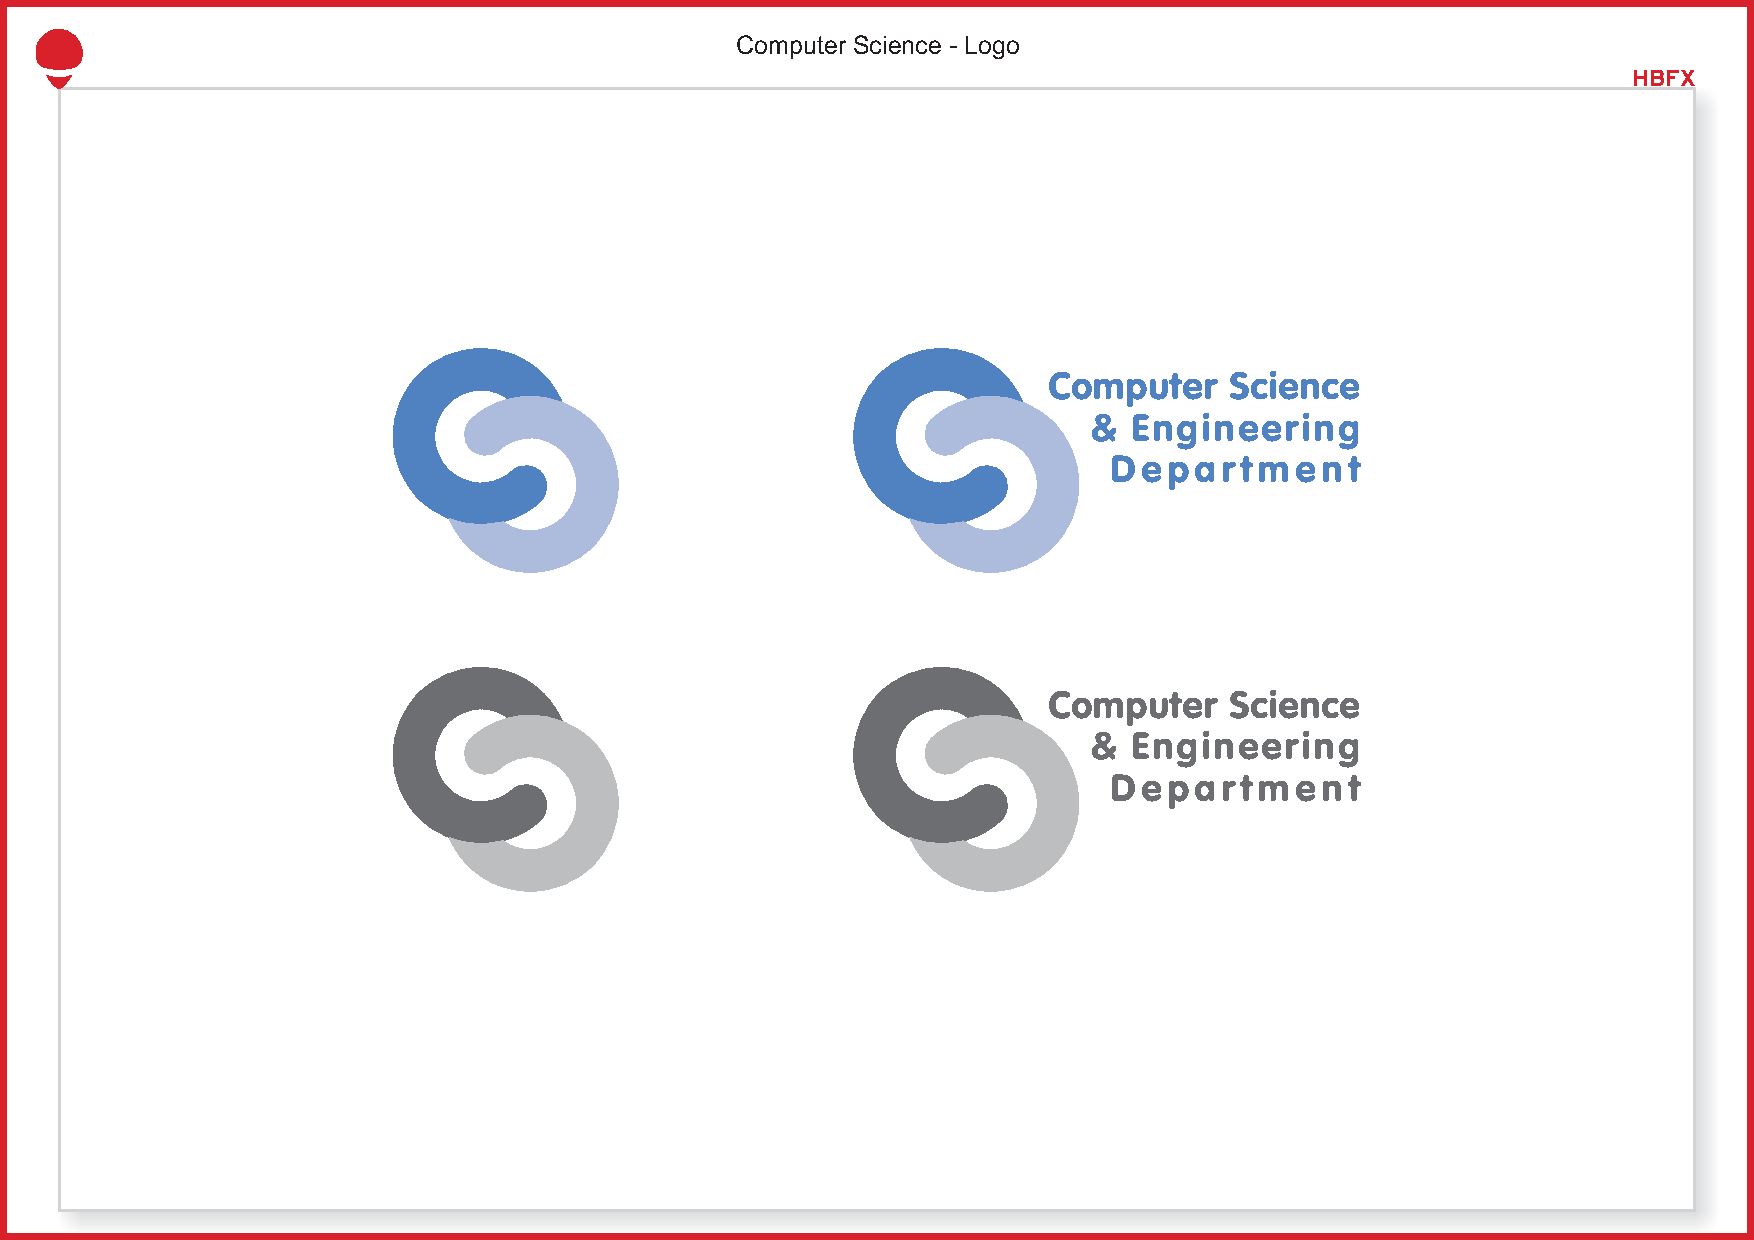
\includegraphics[scale=0.5,trim={14cm 11cm 2cm 5cm},clip=true]{pics/cs-logo.pdf}
\end{tabular}

\vspace{105pt}
{\Huge #2}\\                           % diploma project text
\vspace{40pt}
{\Large #3}\\ \vspace{0pt}  % project title
{\Large #4}\\                          % project subtitle
\vspace{40pt}
{\LARGE \Name}\\                   % student name
\end{center}
\vspace{60pt}
\begin{tabular*}{\textwidth}{@{\extracolsep{\fill}}p{6cm}r}
&{\large\textbf{#5}}\vspace{10pt}\\      % scientific advisor
&{\large \Advisor}                                    % advisor name
\end{tabular*}
\vspace{20pt}
\begin{center}
{\large\textbf{#6}}\\                                % bucharest
\vspace{0pt}
{\normalsize \Year}
\end{center}
\end{titlepage}
}

\newcommand{\frontPageRO}{\frontPage{\UniTextRO}{\DiplomaRO}{\ProjectTitleRO}{\ProjectSubtitleRO}{\AdvisorRO}{\BucRO}}
\newcommand{\frontPageEN}{\frontPage{\UniTextEN}{\DiplomaEN}{\ProjectTitleEN}{\ProjectSubtitleEN}{\AdvisorEN}{\BucEN}}

\linespread{1.15}
\setlength\parindent{0pt}
\setlength\parskip{.28cm}

%% Abstract macro
\newcommand{\AbstractPage}{
\begin{titlepage}
\textbf{\large SINOPSIS}\par
\AbstractRO\par\vfill
\textbf{\large ABSTRACT}\par
\AbstractEN \vfill
\end{titlepage}
}

%% Thank you macro
\newcommand{\ThanksPage}{
\begin{titlepage}
{\noindent \large\textbf{ACKNOWLEDGMENTS}}\\
\Thanks
\end{titlepage}
}



%%%%%%%%%%%%%%%%%%%%%%%%%%%%%%%%%%%%%%%%%%%%%%%%%%   
%%
%%          End of template definitions
%%   
%%%%%%%%%%%%%%%%%%%%%%%%%%%%%%%%%%%%%%%%%%%%%%%%%%


%%% Puteți elimina aceste linii din lucrare, servesc numai pentru template.
\newcommand{\worktype}[1]{[\textit{#1}] }
\newcommand{\dezvoltare}{\worktype{Dezvoltare de produs}}
\newcommand{\cercetare}{\worktype{Cercetare}}
\newcommand{\ambele}{\worktype{Ambele}}
%%%


%%
%%   Campurile de mai jos trebuie modificate de autor. Modificati doar continutul, nu si numele fiecarei definitii
%%
\newcommand{\ProjectTitleRO}{Titlul proiectului de diplomă (ex: Șablon proiect de diplomă)}
\newcommand{\ProjectSubtitleRO}{Subtitlu (ex: versiunea 2018)}
\newcommand{\ProjectTitleEN}{Video Deepfake Detection: Identifying Video Forgeries Through Unimodal and Multimodal Approaches}
%\newcommand{\ProjectSubtitleEN}{Subtitle (eg: 2018 version)}
\newcommand{\Name}{Alexandru Licuriceanu}
\newcommand{\Advisor}{Șl. dr. ing. Dumitru-Clementin Cercel}
\newcommand{\Year}{2027}

% Setări document
\title{Proiect de diplomă}
\author{\Name}
\date{\Year}

%%
%%   Campurile aferente rezumatului
%%
\newcommand{\AbstractRO}{Evoluția rapidă a inteligenței artificiale generative și a modelelor bazate pe difuzie a dus la crearea deepfake-urilor video de înaltă calitate, care prezintă un realism spațial aproape perfect, făcând metodele tradiționale de detecție unimodală (vizuală) din ce în ce mai ineficiente. Tehnicile actuale întâmpină dificultăți în generalizarea rezultatelor pe diverse formate de compresie și modele generative noi. Acest proiect implică cercetarea metodelor actuale, golurile acestora, dar și testarea unor noi metode si modele atât unimodale, cât și multimodale, concepute pentru a detecta clipuri video manipulate, prin identificarea inconsecvențelor semantice între cadre și între fluxurile audio și video.}

\newcommand{\AbstractEN}{The rapid evolution of generative AI and diffusion-based synthesis has led to the creation of high-fidelity deepfakes that exhibit near perfect spatial realism, making traditional unimodal (visual-only) detection methods increasingly ineffective. Current forensic techniques often struggle to generalize across diverse compression formats and novel generative architectures. This research focuses on investigating current state-of-the-art methods, their gaps, but also trying novel methods and models for unimodal and multimodal detection of deepfaked video, through the analyses of semantic inconsistencies, as well as micro-discrepancies between audio and visual streams.}

%%
%%   Campurile aferente paginii de multumiri
%%
\newcommand{\Thanks}{I would like to express my gratitude towards my supervisor, Dumitru-Clementin Cercel, for their guidance and technical insights throughout this research.\\
\\
I would also like to thank the Faculty of Automatic Control and Computers at the National University of Science and Technology POLITEHNICA of Bucharest for providing the computational resources necessary to conduct this study.
}

\begin{document}

\frontPageEN

\begingroup
\linespread{1}
\tableofcontents
\endgroup

\AbstractPage

% poate fi comentata sau stearsa
\ThanksPage


% Textul licentei incepe de aici 



\chapter{Introduction}\pagestyle{fancy}
\section{The Evolution of Generative AI}
The landscape of digital content creation has undergone a paradigm shift over the last decade. Early iterations of deepfakes were primarily made by Generative Adversarial Networks (GANs) \cite{goodfellow2020generative}, which utilized a competitive framework between a generator and a discriminator to synthesize realistic imagery. While revolutionary, GANs often suffered from training instability and mode collapse, frequently leaving behind detectable artifacts such as inconsistent textures or irregular facial landmarks.


However, by 2026, Latent Diffusion Models (LDMs) \cite{rombach2022high} and transformer-based architectures (descendants of Sora and DALL-E) have redefined the state-of-the-art. These models operate by reversing a gradual noise process, allowing for the synthesis of high definition video with unprecedented temporal stability and spatial realism. The result is a generation of synthetic media where the uncanny valley effect has been largely eliminated, rendering traditional forensic methods which rely on identifying pixel-level anomalies increasingly obsolete.


\section{Impact of Deepfake Videos}
The wide-spread availability of high fidelity deepfaking tools has moved the threat from laboratory curiosity to an actual systemic risk. In 2024 and 2025, the global community witnessed the weaponization of deepfakes in political circumstances, where AI-generated content was used to spread misinformation, influence voter sentiment, and impersonate candidates in Romania, Canada, and the United States.

Beyond politics, the financial sector has faced sophisticated social engineering attacks. Notable cases in 2024 involved corporate employees being deceived by real-time deepfake video conferences, leading to multi-million dollar losses. 

This vulnerability occurred in early 2024, involving the Hong Kong office of the multinational engineering company Arup. In this incident, a finance employee was deceived into attending a video conference call where every other participant, including the Chief Financial Officer and several colleagues, was a real-time deepfake.

The attackers utilized publicly available footage to reconstruct the likenesses and voices of the executives, and believing he was following legitimate instructions, the employee executed 15 fraudulent transfers totaling US\$25.6 million \cite{arup2024deepfake}. 



\section{Taxonomy of Video Forgery}
To address the problem of deepfake detection, we must first categorize the methods of manipulation. Video forgeries are no longer monolithic, but rather exist on a spectrum of complexity:
\begin{itemize}
    \item Face-Swap (Identity Swap): The replacement of a target individual’s face with that of a source identity while preserving the original’s movements and environment.
    \item Face Reenactment (Expression Swap): The source actor controls the facial expressions, head movements, and emotions of the target individual.
    \item Lip Syncing (Audio-to-Video): Specifically modifying the mouth region to match a provided audio track, often used to put words into the mouths of public figures.
    \item Fully Synthetic Video: The generation of an entirely non-existent person and environment from a text prompt.
\end{itemize}


\section{The Generalization Gap}
The core motivation for this research lies in the ``Generalization Gap''. Most modern detectors perform exceptionally well on laboratory datasets but fail when faced with in-the-wild content found on social media or forums. Factors such as lossy compression, low lighting, and better generative architectures significantly degrade the accuracy of unimodal, visual-only detectors. The lighting, camera angles, and demographics in training datasets, which are often actors in a studio or laboratory do not reflect the chaotic nature of real-world in-the-wild videos, this being perhaps the most critical failure mode of current forensic systems.


Current research suggests that while a generative model may successfully mimic the visual appearance and movement of a person, it often fails to maintain the complex cross-modal synchronization between the auditory and visual streams. The micro-rhythms of speech, the energy of phonemes, and the corresponding physical deformation of the mouth (visemes) are biologically linked in humans but often mathematically decoupled in AI models. This project proposes that by shifting the focus from pixel analysis to semantic and temporal consistency, and across multiple modalities, we can develop a more robust and future-proof forensic tool.

\chapter{Problem Statement}\pagestyle{fancy}
\section{The Limits of Unimodal Spatial Analysis}
The primary challenge in modern deepfake detection is the obsolescence of spatial artifacts. First-generation manipulation methods usually left visible traces: resolution mismatches between the inserted face and the background, irregular blending boundaries, or unnatural skin textures. In these cases, simple Convolutional Neural Networks (CNNs) could easily classify forged images and videos by detecting high-frequency noise patterns or checkerboard artifacts.

However, the advancements of Latent Diffusion Models (LDMs) and neural rendering techniques in 2025 has largely eliminated these spatial cues. Modern generators synthesize facial features that are statistically indistinguishable from real images at the pixel level. As a result, unimodal detectors that rely on identifying spatial irregularities suffer from a massive performance degradation when applied to quality in-the-wild machine-generated content. Thus, the problem has shifted from identifying visual flaws to identifying semantic flaws within videos.

\section{The Challenge of Cross-Modal Asynchrony}
Although visual generators have spectacular spatial realism, the temporal coherence between the audio and visual streams remains a significant vulnerability. In a genuine video, the production of speech is a complex biomechanical process where the movement of the lips, tongue, and facial muscles (visemes) is tightly coupled with the acoustic signal (phonemes).


The core technical problem is that most deepfake generation pipelines treat audio and video as separate tasks. A Lip-Sync model such as Wav2Lip \cite{wav2lip} or Hallo \cite{xu2024hallo} modifies the mouth region to match an audio track, but often fails to capture the subtle, non-linear dynamics of human speech:
\begin{itemize}
    \item Phoneme-Viseme Mismatch: The model may generate the correct mouth shape for a vowel but fail to close the lips fully for plosive sounds (like ``b'' or ``p'').
    \item Emotional Inconsistency: The audio may carry a tone of anger or urgency, while the eyes and eyebrows remains neutral or static.
\end{itemize}
This cross-modal gap is one of the main problems this research seeks to address. Detecting it requires a model that can analyze both the audio and video streams simultaneously, learning the joint probability distribution of audio-visual events.


\chapter{Related Work}\pagestyle{fancy}
The detection of synthetic media is fundamentally adversarial, being characterized by a continuous arms race between the architectures used to generate forgeries and the  techniques developed to detect them. As generative models have evolved from  Variational Autoencoders (VAEs) and Generative Adversarial Networks (GANs) to modern, high-fidelity Latent Diffusion Models (LDMs), the focus of detection research has necessarily shifted in tandem.


Early literature in this domain predominantly focused on isolating low-level spatial anomalies such as blending boundaries, color disparities, or frequency-domain artifacts left by upsampling layers. However, the contemporary literature (circa 2024–2026) reflects a consensus that spatial-only analysis is no longer sufficient. Consequently, the state-of-the-art has pivoted toward identifying higher-order semantic inconsistencies, specifically temporal irregularities and cross-modal (audio-visual) discrepancies.

This chapter reviews the existing literature on deepfake detection, showcasing the evolution of methodologies from single-modal passive detection to complex, multi-modal fusion frameworks, as well as providing a overview of the publicly available datasets and their benchmarks.

To understand the current challenges in 2026, it is necessary to trace the trajectory of detection methodologies through three distinct generations:
\begin{itemize}
    \item First-Generation (Spatial): Unimodal approaches focusing on frame-level artifacts ( inconsistencies in eye color or background warping).
    \item Second-Generation (Temporal): Sequence-based approaches leveraging Recurrent Neural Networks (RNNs) to identify jitter and temporal discontinuities.
    \item Third-Generation (Multimodal): The current state-of-the-art method, which integrates audio and video streams to detect synchronization anomalies and semantic mismatches.
\end{itemize}

\section{Short Background}
Early forensic methods relied heavily on hand-crafted features. Researchers would manually define specific cues, such as the lack of eye blinking (Li et al., 2018 \cite{li2018exposing}) or unnatural head poses (Yang et al., 2019 \cite{yang2019exposing}) and train simple classifiers like Support Vector Machines (SVMs) to spot them. While effective against primitive deepfakes, these methods proved brittle once the generative models were updated to include blinking (as seen in later versions of DeepFaceLab by Perov et al. \cite{perov2020deepfacelab}), and thus, the detectors became obsolete overnight.

\pagebreak

Consequently, the field pivoted toward data-driven feature extraction using Convolutional Neural Networks (CNNs). Models such as XceptionNet (Chollet et al., 2017) \cite{chollet2017xception}, EfficientNet (Tan et al., 2019) \cite{tan2019efficientnet}, and ResNet (He et al., 2015) \cite{he2015deepresiduallearningimage} became the backbone of modern forensics, learning to identify high-frequency noise patterns invisible to the human eye.

However, as noted by recent surveys (Lin et al., 2024 \cite{lin2024detecting}), these deep learning models suffer from severe overfitting to their training data. A classifier trained on the FaceForensics++ dataset typically sees a performance drop of over 30\% when tested on unseen datasets like DFDC or Celeb-DF, highlighting the critical need for more robust, generalized feature representations.

\section{Datasets and Benchmarks}
The development of robust forensic models is intrinsically linked to the quality and diversity of the datasets available for training. As generative mechanisms have evolved from auto-encoders to complex diffusion-based synthesis, forensic benchmarks have had to adapt to capture increasingly subtle artifacts. This section reviews the progression of deepfake datasets, categorized by their primary modality and generation methodology. A summary of the key statistics is provided in Table \ref{tab:datasets_summary}.

\subsection{Foundational Visual Benchmarks}
FaceForensics++, introduced by Rössler et al. (2019) \cite{rossler2019faceforensics++} established the standard baseline for supervised learning in the domain. The authors compiled 1,000 original video sequences extracted from YouTube and manipulated them using computer-graphics-based approaches like Face2Face (Thies et al., 2016 \cite{thies2016face2face}) and learning-based methods such as NeuralTextures (Thies et al., 2019 \cite{thies2019deferred}). The authors generated a total of 4,000 manipulated videos and provided three levels of compression (Raw, C23, C40) to simulate real-world transmission loss. While FF++ was instrumental in benchmarking early CNN architectures like XceptionNet, its reliance on 2018-era generators means it lacks the high-frequency realism found in modern diffusion outputs.


To address the limitations of scale and diversity, Dolhansky et al. (2020) \cite{dolhansky2020deepfake} released the Deepfake Detection Challenge (DFDC) dataset. Unlike FF++, which used uncontrolled internet videos, Dolhansky et al. recruited 3,426 paid actors to record scenarios with varied lighting, angles, and backgrounds. The dataset comprises over 100,000 clips, making it one of the largest public repositories of synthetic media. However, the authors prioritized scale over uniform quality, as a significant portion of the samples exhibit obvious visual glitches, which allows models to achieve high accuracy without actually learning robust semantic features.

\pagebreak

In contrast to the scale of DFDC, Celeb-DF, presented by Li et al. (2020) \cite{li2020celeb}, focused on visual fidelity. Li et al. collected 590 real YouTube interview videos and generated 5,639 deepfakes using an improved synthesis algorithm designed to reduce the checkerboard artifacts and temporal jitter common in FF++. By smoothing the blending boundaries between the swapped face and the background, Celeb-DF remains a challenging benchmark for visual-only detectors, with many SOTA models dropping from $\sim$99\% accuracy on FF++ to $\sim$65\% on Celeb-DF.

\subsection{Multimodal (Audio-Visual) Datasets}

As the threat landscape shifted towards full-modality synthesis, FakeAVCeleb was introduced by Khalid et al. (2021) \cite{khalid2021fakeavceleb} to facilitate multimodal analysis. Khalid et al. generated 21,566 clips using over 500 distinct celebrities. The primary innovation of this dataset is its fine-grained labeling schema, which categorizes samples into four classes: Real Video-Real Audio, Fake Video-Real Audio, Real Video-Fake Audio, and Fake Video-Fake Audio. This structure allows researchers to train cross-modal networks that can isolate the source of the forgery. However, the audio generation methods used (SV2TTS by Jia et al., 2018 \cite{jia2018transfer}) are now considered relatively low-fidelity compared to modern Voice Conversion models.


To address the data scarcity problem in multimodal forensics, Cai et al. (2025) introduced AVDeepfake-1M++ \cite{cai2025avdeepfake1mlargescaleaudiovisualdeepfake}, currently the largest open-source dataset for audio-visual deepfake detection. The dataset contains over 1.1 million video clips, dwarfing previous benchmarks like FakeAVCeleb, and was constructed by sourcing high-quality videos from YouTube and applying advanced manipulation methods: FSGAN (Nirkin et al., 2019 \cite{nirkin2019fsgan}), Wav2Lip (Liang et al., \cite{liang2024wav2lip}), SV2TTS (Jia et al., 2018 \cite{jia2018transfer}), and Real-Time Voice Cloning (RTVC).


Its primary contribution is the sheer volume of perturbations applied to the data. By including diverse compression levels, noise, and resolution downsampling, AVDeepfake-1M allows models to learn features that are robust to the transmission loss, typical of online platforms.


\subsection{Next-Generation Open-Set Benchmarks}

Hondru et al. (2025) \cite{hondru2025exddv} introduced ExDDV (Explainable Deepfake Detection in Video), the first benchmark specifically designed to train Vision-Language Models (VLMs) for forensic captioning. The dataset aggregates $\sim$5,400 videos from diverse sources including DeeperForensics (Jiang et al., 2020 \cite{jiang2020deeperforensics}) and BioDeepAV (Croitoru et al., 2025 \cite{BioDeepAV2024}), but adds a novel layer of manual annotation: natural language descriptions of the artifacts and pixel-level click maps that pinpoint the exact location of the flaw.

\pagebreak
Croitoru et al. (2025) \cite{croitoru2025mavos} introduced the Multilingual Audio-Video Open-Set Deepfake Detection Benchmark. Recognizing that most datasets are English-centric, Croitoru et al. compiled over 250 hours of video across 8 languages, including Romanian, Mandarin, Hindi, and Arabic. The authors utilized multiple state-of-the-art generators, including EchoMimic (Chen et al., 2025 \cite{chen2025echomimic}), LivePortrait (Guo et al., 2024 \cite{guo2024liveportrait}), and Inswapper/Insightface (Deng et al., 2019 \cite{deng2019arcface, insightface_github}), to create a dataset that specifically targets the language bias in current detectors. Their benchmarks demonstrate that models trained on English data suffer a significant performance degradation when tested on Romanian or Hindi deepfakes due to differences in lip-shape dynamics.

Ciobanu et al. (2026) \cite{ciobanu2025xmad} released the Cross-Domain Multilingual Audio Deepfake Benchmark to address the audio component of the pipeline. Comprising of $\sim$670 hours of speech data (207,000 real and 207,000 fake samples), this dataset enforces a strict cross-domain protocol where the speakers and recording devices in the test set are entirely disjoint from the training set. Ciobanu et al. demonstrated that many existing ``99\% accurate'' audio detectors are merely overfitting to specific speaker identities or channel noise. By aggregating samples from diverse sources and modern vocoders, XMAD-Bench serves as one of the better stress test for the auditory branch of any multimodal system to date.


\begin{table}[htbp]
    \centering
    \caption{Comparative Summary of Forensic Datasets (2019--2026).}
    \label{tab:datasets_summary}
    \resizebox{\textwidth}{!}{%
        \begin{tabular}{l l l l p{6cm}}
            \toprule
            \textbf{Dataset} & \textbf{Year} & \textbf{Modality} & \textbf{Size (Real/Fake)} & \textbf{Primary Contribution} \\
            \midrule
            
            \textbf{FaceForensics++} \cite{rossler2019faceforensics++} & 2019 & Visual & 1K / 4K & Standard baseline for CNNs. \\
            
            \textbf{DFDC} \cite{dolhansky2020deepfake} & 2020 & Visual & $\sim$19K / $\sim$100K & Large scale \& in-the-wild variety. \\
            
            \textbf{Celeb-DF v2} \cite{li2020celeb} & 2020 & Visual & 590 / 5,639 & High visual quality.\\
            
            \textbf{FakeAVCeleb} \cite{khalid2021fakeavceleb} & 2021 & A+V & 500 / $\sim$21K & First multimodal labels (A vs V). \\

            \textbf{AVDeepfake-1M++} \cite{cai2025avdeepfake1mlargescaleaudiovisualdeepfake} & 2021 & A+V & 1M / 1M& Real-world perturbations. \\
            
            \midrule
            
            \textbf{MAVOS-DD} \cite{croitoru2025mavos} & 2025 & A+V & 25K / 35K & Multilingual (8 langs) \& Open-Set. \\
            
            \textbf{ExDDV} \cite{hondru2025exddv} & 2025 & Video+Text & $\sim$1K / $\sim$4.4K & Explainability (XAI) \\
            
            \textbf{XMAD-Bench} \cite{ciobanu2025xmad} & 2026 & Audio & 207K / 207K & Cross-Domain Audio Protocol. \\
            
            \bottomrule
        \end{tabular}%
    }
\end{table}


Collectively, these datasets illustrate a trajectory toward greater complexity and realism. However, a critical gap remains. ExDDV pioneers explainability for visual artifacts and MAVOS-DD addresses multilingual diversity, but there is no single benchmark that combines high-fidelity audio-visual synchronization labels with explainable attention mechanisms. Most current multimodal models function as black boxes, fusing scores without explaining why the audio and video do not match.


\section{Visual-Only Detection Models}
Historically, deepfake detection has been dominated by unimodal visual analysis, focusing on the identification of spatial artifacts such as resolution inconsistencies, blending boundaries, and frequency-domain anomalies left by the generative models used.



\subsection{Frequency-Domain Analysis}
Generative models, particularly those based on Transposed Convolutions, often leave distinct spectral fingerprints that are invisible in the RGB domain but prominent in the frequency domain.

F3-Net (Qian et al., 2020 \cite{qian2020thinkingfrequencyfaceforgery}) is a novel two-stream architecture designed to mine these subtle frequency clues. The model consists of two parallel branches: a standard Xception-based encoder that captures low-level spatial artifacts and a ``Frequency Stream'' branch that applies the Discrete Cosine Transform (DCT) to the input image. Crucially, it employs a learnable frequency filter that adaptively selects the specific frequency bands where the generator's artifacts are most concentrated.


Trained on the FaceForensics++ dataset, F3-Net demonstrated that analyzing the frequency spectrum significantly improves detection accuracy on highly compressed videos (c40 compression), as spectral artifacts are often more resilient to compression than spatial noise.

\subsection{Temporal and Semantic Consistency}
As frame-level image quality improved with the advent of latent diffusion models, spatial artifacts became negligible. Consequently, research shifted focus to temporal incoherence, looking for flickering or unnatural movement of facial features over time.

Haliassos et al. \cite{haliassos2021lips} introduced a semantic-level detection approach that targets the high-level inconsistencies in mouth movements. The core hypothesis is that while a generator can synthesize realistic skin texture, it struggles to replicate the complex, biologically constrained dynamics of human speech. This model is presented in Figure \ref{fig:haliassos}:

\begin{figure}[htbp]
    \centering
    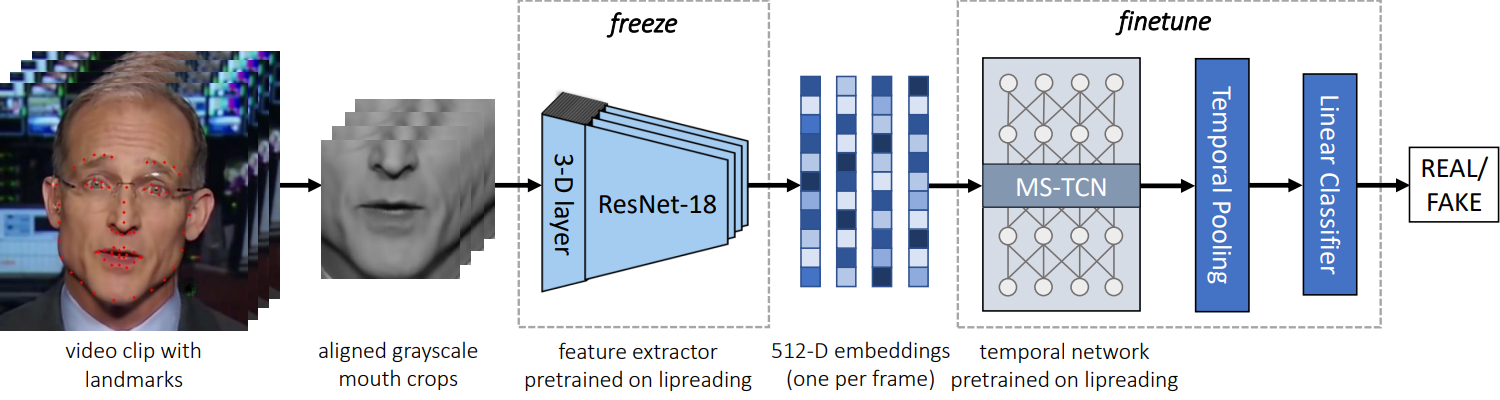
\includegraphics[width=1.0\textwidth]{related_work/haliassos.PNG} % Replace with your file name
    \caption{Overview of the finetuning phase on face forgery detection. Source: ``Lips Don’t Lie: A Generalisable and Robust Approach to Face Forgery Detection'' by Haliassos et al. \cite{haliassos2021lips}.}
    \label{fig:haliassos} % Unique label for referencing (e.g., see Figure \ref{fig:my_label})
\end{figure}



The model leverages a pretrained lip-reading network (ResNet-18 + MS-TCN) originally designed for visual speech recognition. By freezing the feature extractor, LipForensics forces the detector to learn high-level semantic irregularities rather than overfitting to low-level pixel noise.
Evaluation on FaceForensics++ and Deepfake Detection Challenge (DFDC) showed that LipForensics achieves SOTA generalization to unseen manipulation methods, as the biological constraints of speech are universal across all generators.


Zheng et al. \cite{zheng2021exploring} proposed FTCN (Fully Temporal Convolution Network), a specialized temporal transformer to detect temporal flickering. Unlike standard 3D-CNNs, FTCN utilizes a temporal transformer module to model long-range dependencies in the video sequence. It explicitly minimizes the temporal coherence of the features, operating on the assumption that real video has smooth, continuous transitions, whereas deepfakes exhibit microscopic temporal discontinuities.


\subsection{Diffusion-Specific Reconstruction}
The emergence of diffusion models introduced a new class of ``noise-based'' artifacts distinct from GANs.

DIRE (Diffusion Reconstruction Error) is a model introduced by Wang et al. (2023) \cite{wang2023dire} that utilizes a generative detection method based on the hypothesis that images generated by a diffusion model are easier for a diffusion model to reconstruct. The input image is essentially reverse-diffused (DDIM inversion) to obtain its latent noise, and then reconstructed.
 The difference/error between the original image and the reconstructed image serves as the detection signal. Real images have high reconstruction error, making them hard to approximate, while deepfakes have low error.

Addressing the slow inference speed of DIRE, Chu et al. (2025) \cite{chu2025fire} proposed FIRE (Frequency-Guided Reconstruction), which applies the reconstruction process only to specific high-frequency bands where diffusion models are known to hallucinate texture details. This optimization makes it feasible for real-time video analysis while maintaining robust detection rates against 2026-era generators like Sora, Kling and Veo.


\section{Multimodal Detection Methods}
Multimodal learning represents the current state of deepfake detection. Unlike unimodal approaches that struggle with high-fidelity synthesis in a single domain, multimodal frameworks exploit the semantic and temporal correlations between auditory and visual streams. The core idea is that while generative models can synthesize realistic faces and clone voices, maintaining the subtle, non-linear synchronization between phonemes and visemes still remains a significant challenge.

\subsection{Naive Fusion Strategies}
Mittal et al. (2020) \cite{mittal2020emotions} utilized a ``late fusion'' approach where separate Siamese networks processed audio and video to detect emotion. The final classification was a simple weighted average of the two probability scores. While effective for obvious mismatches such as a happy voice with a sad face, this method fails to capture fine-grained temporal asynchrony.

\begin{figure}[htbp]
    \centering
    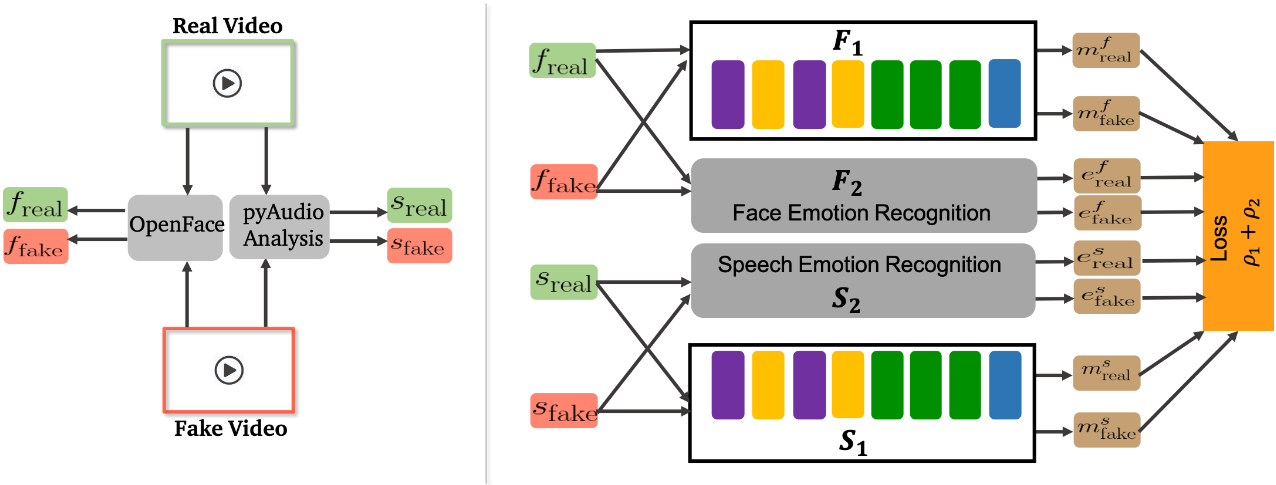
\includegraphics[width=1.0\textwidth]{related_work/mittal.PNG} % Replace with your file name
    \caption{Training Routine:  We extract facial and speech features from the raw videos (left). Theextracted features are passed to the training network that consists of two modality embedding net-works and two perceived emotion embedding networks (right). Source: ``Emotions Don’t Lie: An Audio-Visual Deepfake Detection Method using Affective Cues'' by Mittal et al. \cite{mittal2020emotions}.}
    \label{fig:mittal} % Unique label for referencing (e.g., see Figure \ref{fig:my_label})
\end{figure}


A key limitation of naive fusion is modality dominance, where the model over-relies on the stronger modality, usually video, and ignores the audio. To counter this, the authors used modality dropout, which randomly zeros out one stream during training, forcing the network to learn robust features from both independently.


\subsection{Cross-Modal Attention and Explainability}
The state-of-the-art methods utilize transformers to learn the correlation between modalities at every time step. This allows for Cross-Modal Attention, where the audio stream can attend to specific visual regions and vice-versa.

Zhou et al. (2021) \cite{zhou2021joint}, propose a novel stream framework that exploits the inherent synchronization between visual and audio modalities to identify forged content. The architecture consists of independent video and audio streams, utilizing an R(2+1)D-18 backbone for visual inputs and a 1D convolutional network for raw waveforms, bridged by a third sync-stream that learns the correspondence between speech phonemes and lip visemes.

This sync-stream uses central connections to fuse features from both modalities at multiple layers, using strided convolution and tiling operations to align the temporal dimensions of audio and video features. To further refine this alignment method, the authors implement an inter-attention mechanism that weighs features based on cross-modality relevance.


\begin{figure}[htbp]
    \centering
    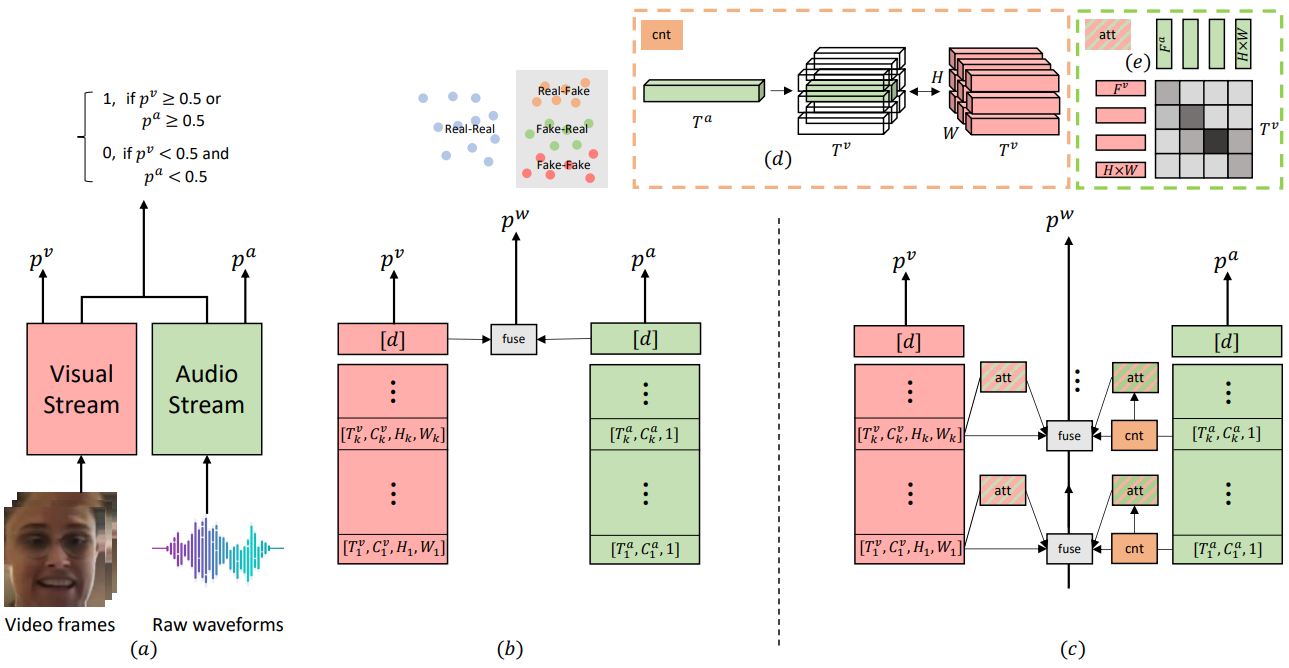
\includegraphics[width=1.0\textwidth]{related_work/zhou.PNG} % Replace with your file name
    \caption{Overview of proposed frameworks. (a) Independently trained prediction framework. $p^v$ and $p^a$ are outputs for video and audio streams, representing the probability of the input being fake. (b) Late-fused joint prediction network with $p^w$ denoting the probability of the whole video being modified and $[d]$ denoting last layers of networks where representations are spatiotemporally pooled. (c) Two-plus-one joint detection framework. Source: ``Joint Audio-Visual Deepfake Detection'' by Zhou et al. \cite{zhou2021joint}.}
    \label{fig:zhou} % Unique label for referencing (e.g., see Figure \ref{fig:my_label})
\end{figure}




Analysis using ScoreCAM visualization reveals that while independent detectors often focus broadly on facial textures or eyes, this joint framework specifically localizes artifacts in the mouth region, confirming its ability to detect lip-sync inconsistencies.



Wu et al. (2025) \cite{wu2025hola} proposed HOLA, which unlike previous architectures that process audio-visual streams in a single pass, HOLA introduces an iterative-aware cross-modal learning module. This mechanism repeatedly refines the feature alignment between the audio and visual encoders, allowing the model to progressively denoising the synchronization signals before making a decision.

\begin{figure}[htbp]
    \centering
    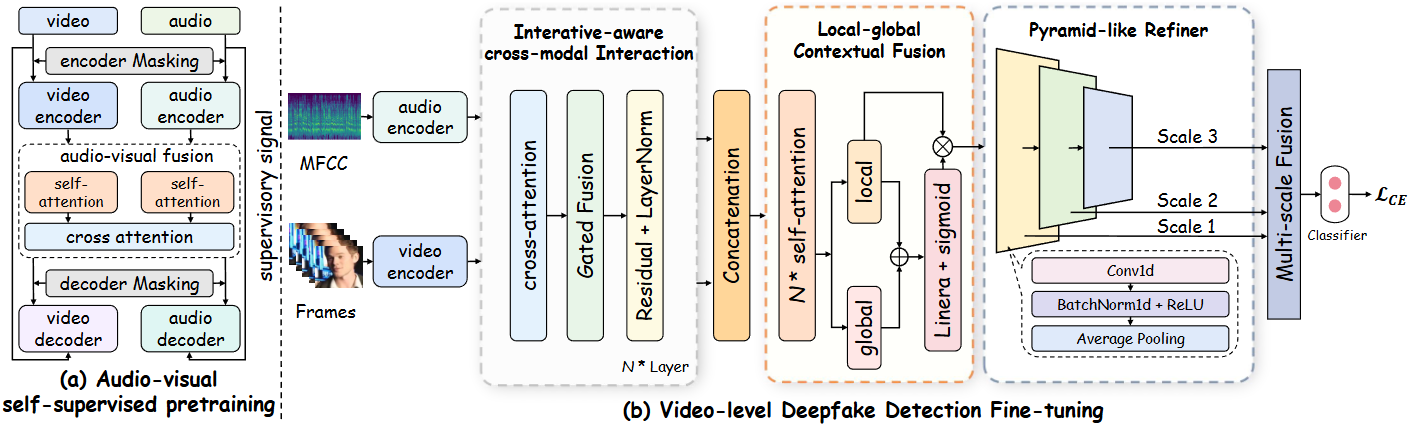
\includegraphics[width=1.0\textwidth]{related_work/wu.PNG} % Replace with your file name
    \caption{ The overall illustrations of introduced HOLA. Source: ``HOLA: Enhancing Audio-visual Deepfake Detection via Hierarchical Contextual Aggregations and Efficient Pre-training'' by Wu et al. \cite{wu2025hola}.}
    \label{fig:wu} % Unique label for referencing (e.g., see Figure \ref{fig:my_label})
\end{figure}


Furthermore, to address the limitation of fixed-window analysis, the authors implemented a Hierarchical Contextual Modeling block that aggregates features at multiple temporal scales, from local frame-level jitter to global video-level semantic consistency. By pre-training on a massive corpus of 1.81 million samples, HOLA demonstrated that learning multi-scale temporal dependencies is critical for detecting high-fidelity forgeries that maintain perfect lip-sync in short segments but fail to preserve long-term behavioral coherence. The complete architecture is presented in Figure \ref{fig:wu}.


Hong et al. introduce a unified framework designed to tackle three distinct subtasks: deepfake classification, localization of forged facial components, and identifying the sequential order of manipulations. The system's architecture utilizes a CNN-transformer network. A CNN backbone extracts spatial features, which are then processed alongside learnable class tokens by a Transformer encoder to capture both local artifacts and global facial correlations.

For binary classification, the model treats an image as a ``bag'' and its feature map pixels (patches) as ``instances''. It employs a contrastive MIL loss ($\mathcal{L}_{CLS}$) that estimates the probability of an image being fake by identifying at least one manipulated patch, effectively distinguishing genuine images from forged ones. To localize specific forged components and recover their manipulation order, the authors formulate the problem as a ranking task. They design a specialized ranking loss ($\mathcal{L}_{Rank}$) that ensures the predicted probabilities for various facial labels respect the ground-truth sequence of modifications. This whole process is presented in Figure \ref{fig:hong}:

\begin{figure}[htbp]
    \centering
    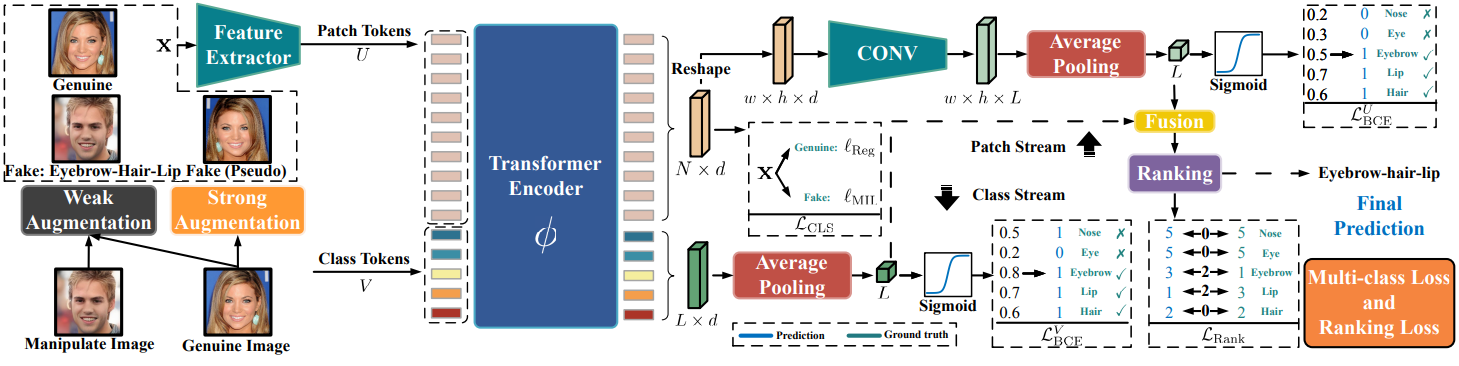
\includegraphics[width=1.0\textwidth]{related_work/hong.PNG} % Replace with your file name
    \caption{The model architecture. There are two types of input tokens: patch tokens extracted from CNN+FPN and learnable class tokens. The stage of model training is driven by three loss terms: $\mathcal{L}_{CLS}$, $\mathcal{L}_{BCE}$ and $\mathcal{L}_{Rank}$ to achieve contrastive multiple instance learning, multi-label localization and ranking, respectively. In the inference stage, the sequential order of deepfake manipulations can be readily obtained from the rank order of the output multi-label probabilities. Source: ``Contrastive Learning for DeepFake Classification and Localization via Multi-Label Ranking'' by Hong et al. \cite{hong2024contrastive}.}
    \label{fig:hong} % Unique label for referencing (e.g., see Figure \ref{fig:my_label})
\end{figure}

\section{Conclusion}
The state-of-the-art has clearly moved towards audio-visual analysis, where frameworks such as HOLA demonstrate that while generative models can synthesize photorealistic visual fidelity, they struggle to maintain the intricate biomechanical synchronization between phonemes and visemes over extended temporal windows.

However, despite these advancements, a separation persists between high-performance black-box systems and interpretable but less accurate forensic tools. Most current multimodal architectures require prohibitive computational resources or fail to provide granular explanations for their decisions.

\section{Future Directions}
Building upon the gaps identified in current state-of-the-art methods, this research proposes a comprehensive evaluation of multimodal forensic architectures on the newly released MAVOS-DD and ExDDV datasets. MAVOS-DD will serve as the primary testbed for assessing generalization across linguistic barriers, specifically testing whether cross-modal synchronization features learned from English-centric data can robustly detect forgeries in under-represented languages such as Romanian. Concurrently, ExDDV will be utilized to benchmark the explainability of the models, shifting the evaluation metric from simple binary accuracy to the precision of pixel-level localization and natural language justification.

Our tests will include testing the MAVOS-DD dataset on a simpler network such as the one presented by Mittal et al. \cite{mittal2020emotions}, then on a more complex network, FTCN by Zheng et al. \cite{zheng2021exploring}. Finally, we will be benchmarking both MAVOS-DD and ExDDV on existing state-of-the-art methods such as the one proposed by Hong et al. \cite{hong2024contrastive}, capable of detection as well as localization.

Furthermore, we will propose an experimental framework that will integrate the hierarchical attention mechanisms of HOLA with the localization objectives of Hong et al. into a unified architecture. By injecting an auditory stream into the ranking mechanism, this approach aims to determine if a single model can achieve high-fidelity detection on the multilingual challenges of MAVOS-DD, and if using the audio of the samples helps or hinders performance, while simultaneously providing the granular, human-interpretable explanations required by the ExDDV benchmark.


% Asa se specifica folosirea unui fisier cu referinte bibliografice:
\bibliographystyle{plain}
\bibliography{bibliography}

%% O alta varianta ar fi fost includerea de articole direct in acest fisier
%% in felul urmator:
%% \begin{thebibliography}{ABC}
%%
%% \bibitem{article}
%%  H. Baali, H. Djelouat, A. Amira and F. Bensaali,
%%  ``Empowering Technology Enabled Care Using IoT and Smart Devices:
%   A Review''. In: IEEE Sensors Journal, vol. 322 (10), pp. 891--921, 1905.
%%
%% (more \bibitem items here...)
%%
%% \end{thebibliography}

%% Daca vreti ca o sectiune sa inceapa pe o pagina noua, puteti forta acest lucru cu comanda "\newpage", ca mai jos:

%\newpage

% \chapter*{Anexe}\addcontentsline{toc}{chapter}{Anexe}

% Anexele sunt opționale.
% Ce poate intra în anexe:
% \begin{itemize}
% \item	Exemplu de fișier de configurare sau compilare;
% \item	Un tabel mai mare de o jumătate pagină;
% \item	O figura mai mare mai mare de jumătate pagină;
% \item	O secvență de cod sursa mai mare de jumătate pagină;
% \item	Un set de capturi de ecran (``screenshot''-uri);
% \item	Un exemplu de rulare a unor comenzi plus rezultatul (``output''-ul) acestora;
% \item 	În anexe intră lucruri care ocupă mai mult de o pagină ce ar întrerupe firul natural de parcurgere al textului.
% \end{itemize}

% \begin{appendices}

% \chapter{Extrase de cod} % Introduce o nouă anexă
% \ldots


% \end{appendices}
\end{document}